
\fullcite{mure05}

%..............................
\paragraph{Constitutive models}.

\begin{multicols}{2}
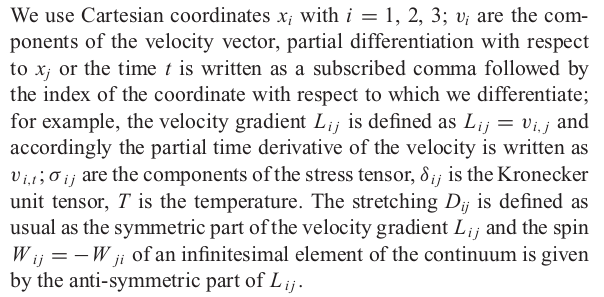
\includegraphics[width=8cm]{images/viscoelasticity/mure05a}\\
\end{multicols}

\begin{multicols}{2}
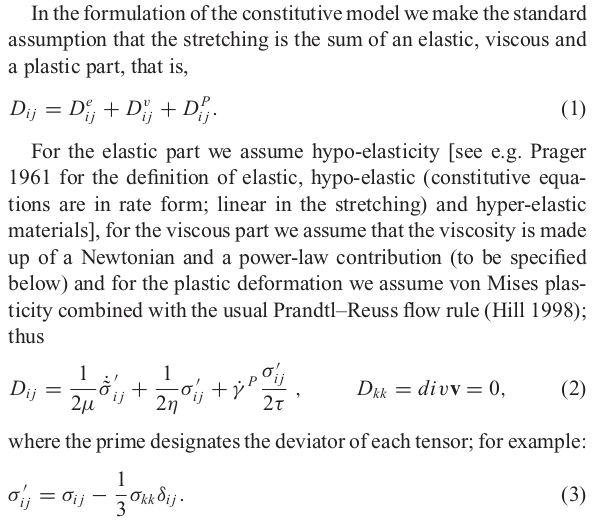
\includegraphics[width=8cm]{images/viscoelasticity/mure05b}\\
\[
\dot{\bm\varepsilon} = 
\dot{\bm\varepsilon}^e +
\dot{\bm\varepsilon}^v +
\dot{\bm\varepsilon}^p 
\]
\[
\dot{\bm\varepsilon}=\frac{1}{2\mu} \frac{{\cal D}{\bm\tau}}{{\cal D}t} 
+ \frac{1}{2\eta} {\bm \tau} + \dot{\gamma}^p \frac{{\bm \tau}}{\tau_e}
\]
\[
{\rm tr}(\dot{\bm\varepsilon} = {\rm div}(\vec\upnu)= 0 
\]
\end{multicols}

\begin{multicols}{2}
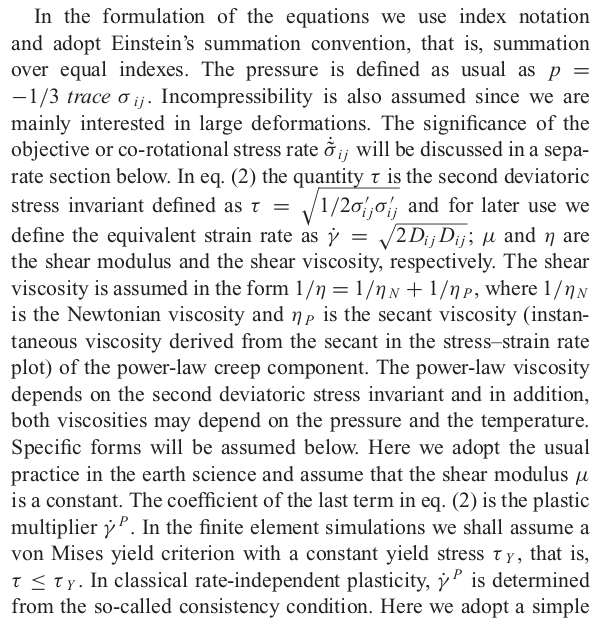
\includegraphics[width=8cm]{images/viscoelasticity/mure05c}\\
\[
p=-\frac13 {\rm tr}({\bm\sigma})
\]
\end{multicols}

\begin{multicols}{2}
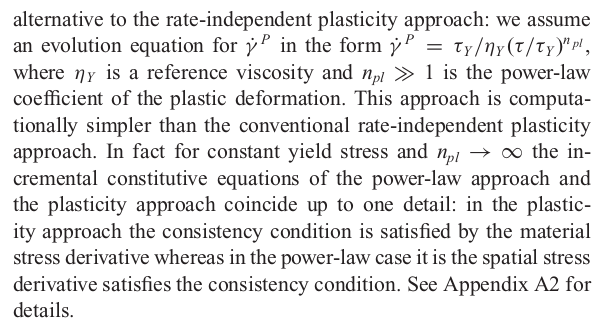
\includegraphics[width=8cm]{images/viscoelasticity/mure05d}\\
\[
\dot\gamma= \frac{\tau_y}{\eta_y} \left(\frac{\tau_e}{\tau_y}\right) ^{n_{pl}} 
\]
where $\eta_y$ is a reference viscosity and $n_{pl}>>1$ is the 
power-law coefficient of the plastic deformation.
\end{multicols}

\begin{multicols}{2}
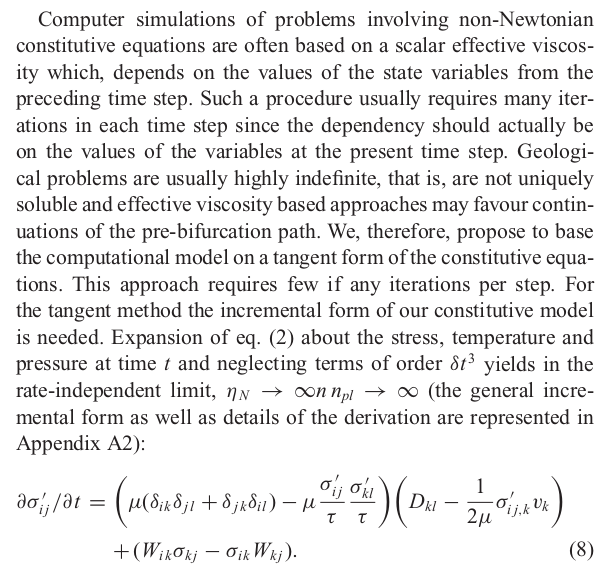
\includegraphics[width=8cm]{images/viscoelasticity/mure05e}\\
\[
 = ... \dot{\bm\omega}\cdot {\bm\sigma} - {\bm\sigma}\cdot \dot{\bm\omega}
\]
whaaat ??!?
\end{multicols}

\begin{multicols}{2}
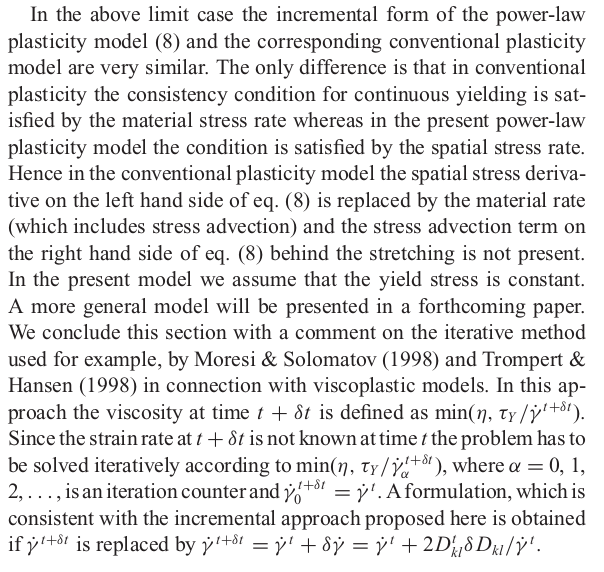
\includegraphics[width=8cm]{images/viscoelasticity/mure05f}\\
\end{multicols}

\newpage
%..................................
\paragraph{Objective stress rates}.

\begin{multicols}{2}
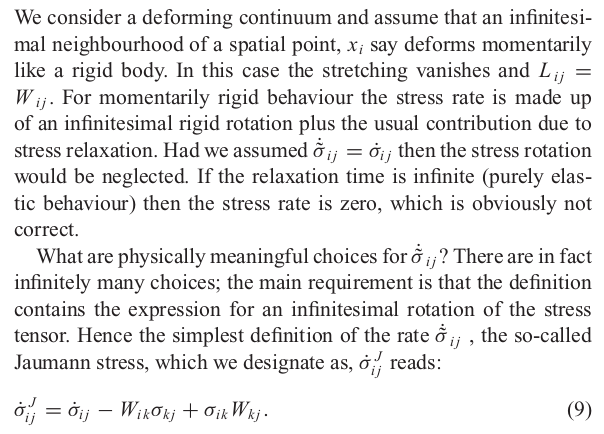
\includegraphics[width=8cm]{images/viscoelasticity/mure05g}\\
\end{multicols}

\begin{multicols}{2}
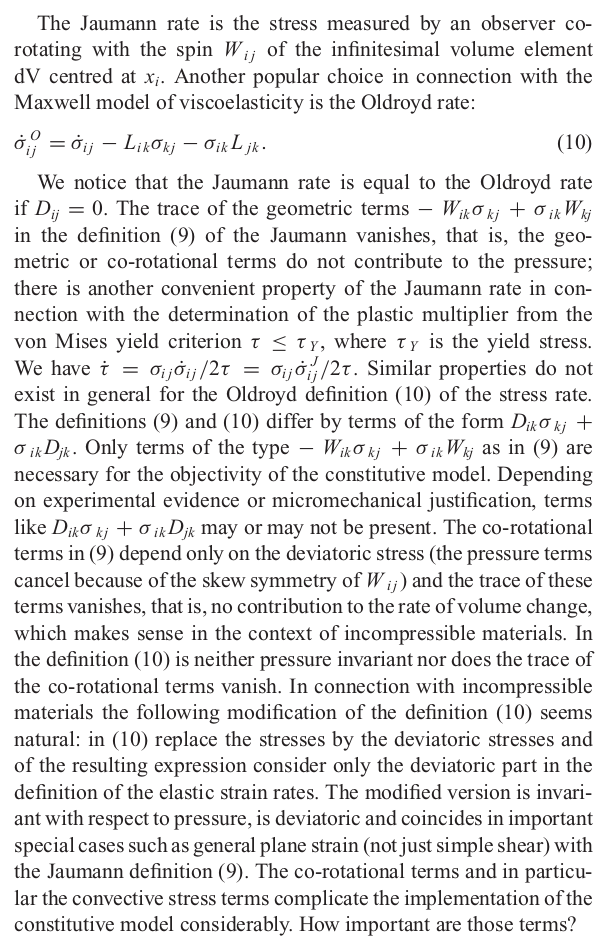
\includegraphics[width=8cm]{images/viscoelasticity/mure05h}\\
\end{multicols}

\begin{multicols}{2}
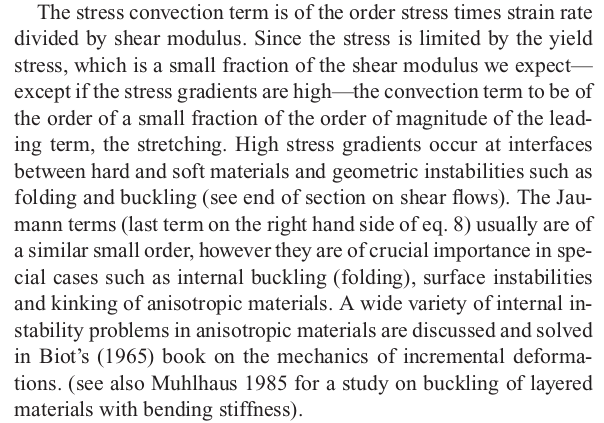
\includegraphics[width=8cm]{images/viscoelasticity/mure05i}\\
\end{multicols}

\begin{multicols}{2}
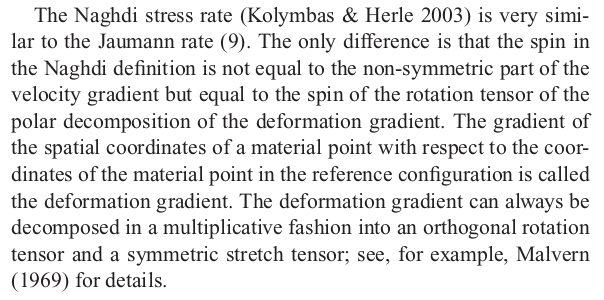
\includegraphics[width=8cm]{images/viscoelasticity/mure05j}\\
\end{multicols}

\begin{multicols}{2}
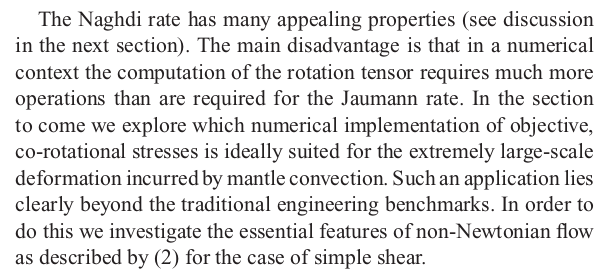
\includegraphics[width=8cm]{images/viscoelasticity/mure05k}\\
\end{multicols}






